\chapter{Implementation}
\section{Julia}
\label{sec:Julia}
Julia is a new programming language that was created by Jeff Bezanson, Alan Edelman, Stefan Karpinski and Viral B. Shah  at MIT, Massachusetts Institute of Technology \emph{\citep{juliaLab}}. The language was created in 2009, but was first released publicly in 2012. In 2012 the creators said in a blog post that
\begin{quotation}
"We want a language that’s open source, with a liberal license. We want the speed of C with the dynamism of Ruby. We want a language that’s homoiconic, with true macros like Lisp, but with obvious, familiar mathematical notation like Matlab. We want something as usable for general programming as Python, as easy for statistics as R, as natural for string processing as Perl, as powerful for linear algebra as Matlab, as good at gluing programs together as the shell. Something that is dirt simple to learn, yet keeps the most serious hackers happy. We want it interactive and we want it compiled. (Did we mention it should be as fast as C?)"\emph{\citep{juliaBlogRelease2012}} .
\end{quotation}
So in short, it seems to be the perfect language for numerical applications and it would be interesting to see how it performs compared to MATLAB. When it comes to AD in Julia, there are already some packages that can be used. Most of them are backward AD packages designed for machine learning like for example AutoGrad \emph{\citep{knet2016mlsys}} and Zygote \emph{\citep{innes2018don}}. The reason why AD-packages for machine learning are based on backward AD is that, without going to deep into what it consist of, it largely consist of minimisation of functions with a large number of input parameters, but with only one output parameter. As discussed in \autoref{sec:BackwardAD}, backward AD is much more efficient than forward AD in these type of evaluations. But there is one package called ForwardDiff \emph{\citep{ForwardDiff}} that uses forward AD and is being developed by the Julia community. This package works very well for some applications, but for others it has some limitations that are not ideal, i.e., 
\begin{itemize}
    \item The function we want to differentiate only accepts a single argument. This is possible to work around such that if you have vector function $f$ with input parameters $x,y,z \in \Re^n$ you can merge them into one vector of length $3n$ and then obtain the Jacobian. Although this works and you get the correct answer, it is not optimal as you could have to make local workarounds to make the code work and this will cause unreadable code.
    \item The function we want to differentiate must be on the form of a generic Julia function, i.e., $g(x) = 3x.*x$. Here $x.*x$ symbolize elementwise multiplication. This means that if we have a function like $h(x) = 3x.*x + \text{sum}(x)$, where all elements in $g(x)$ are added with the sum of all elements in $x$, it will not be possible to use ForwardDiff to obtain the Jacobian.
    \item The Jacobian calculated by ForwardDiff is a full matrix. In some calculations when the Jacobian is dense anyway, this will not have any major adverse effects, but in many numerical applications, the Jacobian will be sparse. By representing a sparse matrix on a full matrix format, we will loose a lot of potential computation efficiency.
\end{itemize}

\section{Implementation of Automatic Differentiation}
When it comes to implementing AD there are two major concerns. First is that it must be easy and intuitive to use, the second is that it must be efficient code as it will be used in computational demanding calculations. A convenient way to store the AD-variables in Julia is to make a structured array (\texttt{struct}) that has two member variables, \texttt{val} and \texttt{jac}, that stores respectively the value and the corresponding Jacobian. 
\lstinputlisting{code/AD_struct.jl} 
The struct is mutable such that we are able to change the values of the struct after it is defined. The \texttt{val} variable is a vector unless it is a scalar variable, then it is only of type  \texttt{Float64}. When it comes to the Jacobian there are multiple ways of storing the matrix. Depending on the application and how much, and what type of, manipulation of the matrix you are going to do, the choice is based on efficiency and convenience. My implementation is inspired by the implementation in MRST \emph{\citep{lieMrstUrl}} where we represent the Jacobian \texttt{jac} as a vector of sparse matrices, where each sparse matrix is the Jacobian w.r.t. each primary variable. This implementation gives the freedom to easily work with the Jacobian for just a single primary variable.

Now we need to implement operators for this type of struct. The importance of the way you implement the AD operators and elementary functions can be expressed in a short example: Assume you have two variables $x$ and $y$ and that you want to compute the function $f(x,y) = y+\exp(2xy)$. If the implementation is based on making new functions that take in AD-variables as input parameters, it will for the evaluation of $f$ look something like this: 
\begin{center}
    $f$ = \texttt{ADplus}($y$,\texttt{ADexp}(\texttt{ADtimes}(2,\texttt{ADtimes}($x,y$)))).
\end{center}
This is clearly not a suitable way to implement AD and should be avoided. Lie and Neidinger suggests in \emph{\citep{lieMrstUrl}} and \emph{\citep{doi:10.1137/080743627}} a much more elegant implementation where instead of making new functions that take in AD-variables as parameters, one should overload the standard operators (+,-,*,/) and the elementary functions (exp, sin, log, etc.). In Julia this can be done by exploiting the fact that Julia has \emph{multiple dispatch}. A quick explanation that satisfies our needs is that at runtime, the compiler understands what types are given as input for either a operator or a function and chooses the correct method based on this. This is done by implementing a function \lstinputlisting{code/overload_plus_operator_AD.jl} 
that overloads the + operator. Here, we import the + operator from Base (which is where the standard functions in Julia lie) and overload it for AD variables. This means that it is only when there are AD variables on both sides of the operator that this implementation is used. Hence, if I declare $x = 1$, $y = 3$ and then $z = x+y$, Julia understands that it is not the definition above, but the normal addition for integers it should use. But if we declare $x,y = \texttt{initialize\_AD}(1,3)$ such that $x$ and $y$ both are AD variables, then when we write $z = x+y$, Julia's multiple dispatch will understand that it is our definition of the "+" operator that is meant to be used. What we need to remember is that if I now write $z = x + 3$, with $x$ as an AD variable, Julia will deploy an error message. This is because we also have to implement
\lstinputlisting{code/overload_plus_operator_number.jl}
Here, the first function will be used if the + operator is used with an AD variable on the left hand side and a number on the right. The last line is a compact way of writing the opposite function which will be used when the number is on the right hand side. But as you can see, we do not implement the same thing twice, we use the function we already have made. When we have implemented all the function necessary it gives us the opportunity for the function $f$ above to only write $f = y+\exp(2*x*y)$ and Julia will understand that it is our implementation of +, * and exp that shall be used, and $f$ will become an AD-variable with the correct value and derivatives. 

Another advantage of Julia's multiple dispatch system is clear if we look at how we can overload the \texttt{sum} function. One might think that we would try something like
\lstinputlisting{code/overload_sum.jl}
which would indeed work, but to exploit Julia's multiple dispatch fully, we can instead overload the \texttt{iterate} function. This function explains how we shall iterate through an AD variable. 
\lstinputlisting{code/iterate.jl}
Now, the built-in \texttt{sum} function will work on AD variables since it knows how to iterate through the variable and when it adds up the values, the + operator we defined above is being used. And not only that! All built-in functions that iterate through the input will also work (given that the functions they use on the variable also are overloaded). As an example, if we now overload the elementary operation /, the Base function \texttt{mean} will also work on AD variables.
\todo[inline]{Write about the dot-operator \cite{JuliaIssueDot}}
\section{Benchmark of Automatic Differentiation}
As mentioned in \autoref{sec:Julia}, Julia already has an AD library called ForwardDiff \emph{\citep{ForwardDiff}} that uses forward AD. Hence, it would be interesting to see how the two implementations compare when the functions evaluated are getting larger. As another reference, I have added the AD implementation in the MATLAB Reservoir Simulation Toolbox (MRST) \emph{\citep{mrstHomepage}} to the benchmark, to see how the Julia implementations compare to an optimized AD tool in MATLAB. To benchmark the efficiency of the different AD tools, I have evaluated the vector function $f: \Re^{n\times 3} \rightarrow \Re^n $ where
\begin{equation}
\label{eq:benchmarkFunction}
f(x,y,z)  = \exp(2xy) - 4xz^2 + 13x - 7,
\end{equation}
and $x,y,z \in \Re^n$. \autoref{fig:benchmarkAD} shows how time spent calculating the function value and the Jacobian of the function, for the different methods, scales as the length of the vectors $n$ increases.
\begin{figure}[htbp]
    \centering
    \begin{subfigure}[t]{0.48\textwidth}
        \centering
        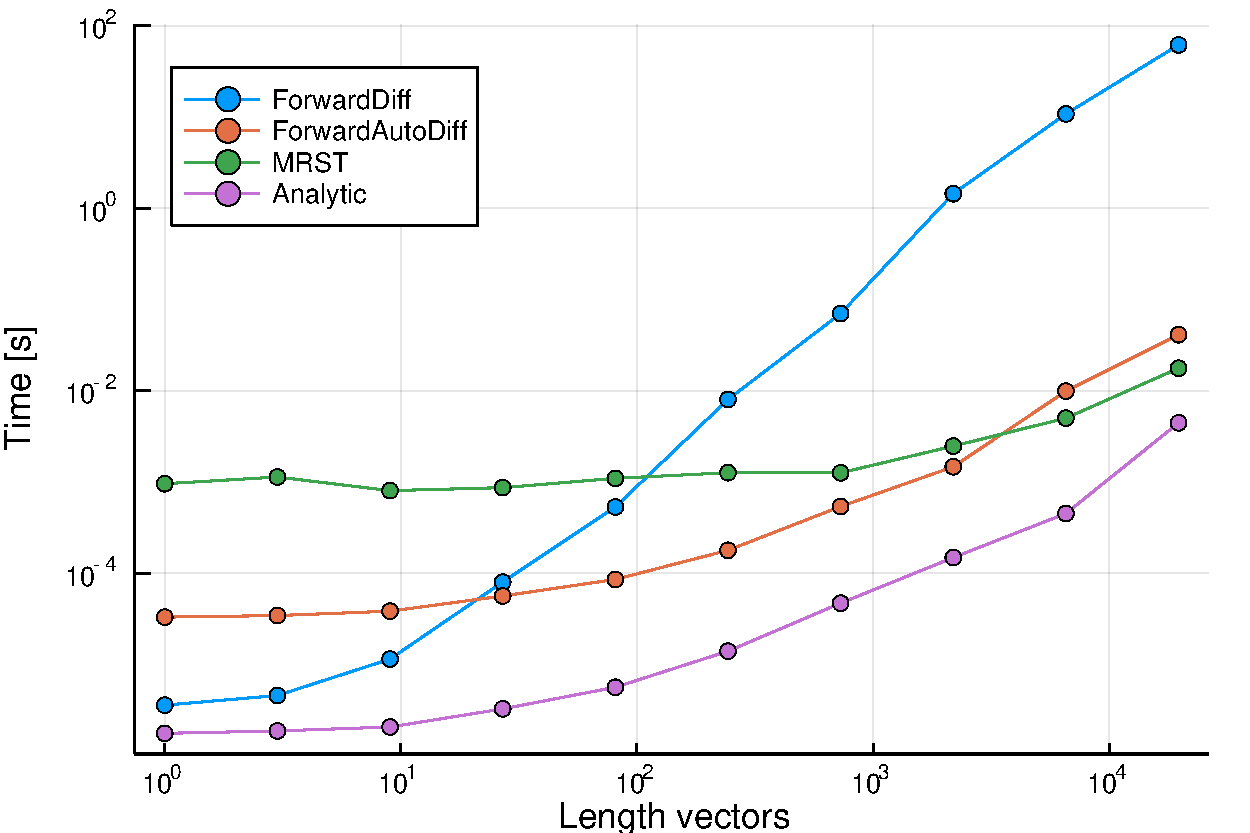
\includegraphics[width = \textwidth]{figures/benchmark_all_ADs.pdf}
        \caption{}
        \label{fig:benchmarkAllADs}
    \end{subfigure}
    \begin{subfigure}[t]{0.49\textwidth}
        \centering
        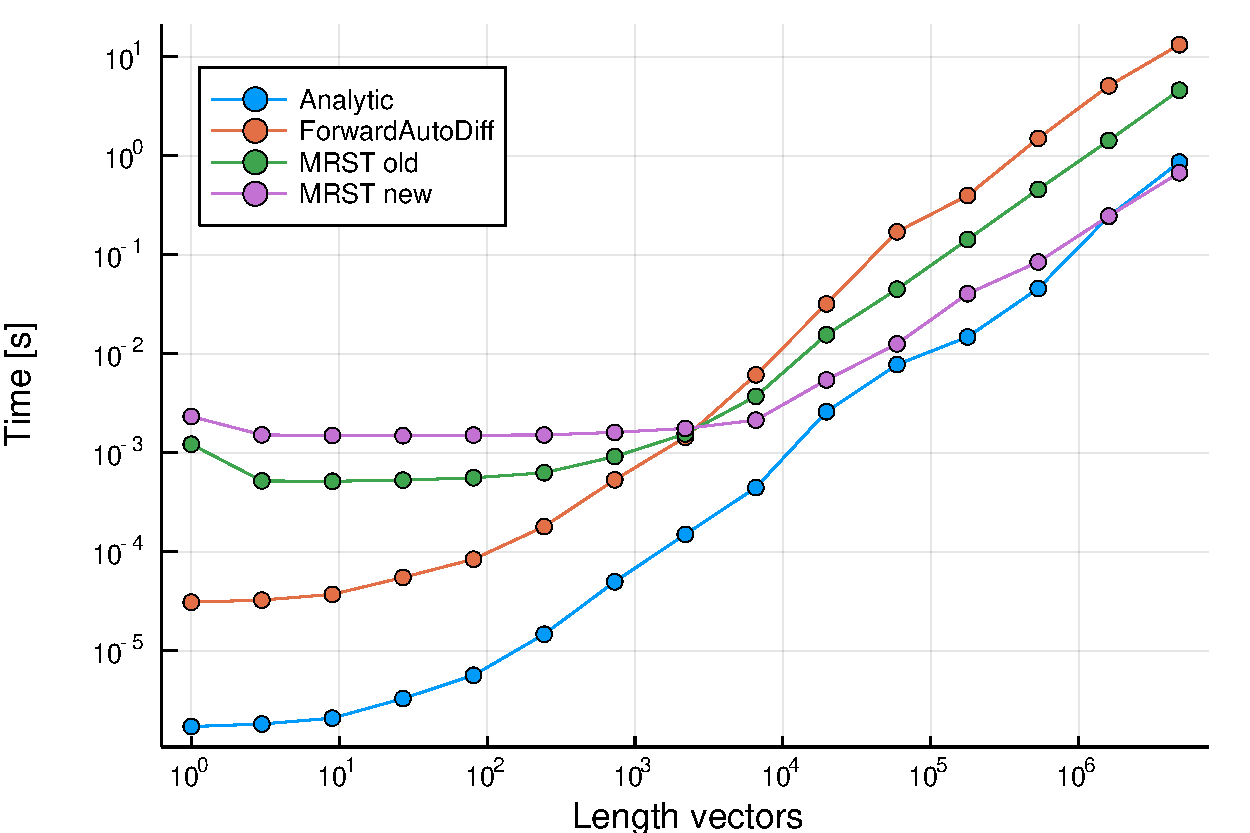
\includegraphics[width = \textwidth]{figures/benchmark_long_vectors_4.pdf}
        \caption{}
        \label{fig:benchmarkLongVectors}
    \end{subfigure}
    \caption{Time spent calculating the value and Jacobian of $f$ in \eqref{eq:benchmarkFunction} as a function of length of the input vectors.}
    \label{fig:benchmarkAD}
\end{figure}
In \autoref{fig:benchmarkAllADs} we have four different graphs. The analytic graph is simply the evaluation the analytic functions $f(x,y,z)$, $f_x$, $f_y$ and $f_z$. ForwardDiff is the AD package in Julia, MRST is the AD tool implemented in MATLAB and ForwardAutoDiff is the AD tool I have implemented in Julia. The first thing you observe is that ForwardDiff scales very badly as n becomes large. This is because it creates and works with the full Jacobian matrix as discussed in \autoref{sec:Julia}. For $f(x,y,z)$ this will be a $3n \times 3n$ matrix which is a matrix with more than 3 billion elements for the largest values of $n$. We can also observe that for small vectors, MRST and ForwardAutoDiff have much more overhead than ForwardDiff and the analytic solution and hence are slower, but as $n$ grows, this overhead becomes more negligible. 

The computational costs of both MRST and ForwardAutoDiff approach the analytic evaluation as $n$ grows, and it is thus interesting to see how they scale for even larger $n$. This can be seen in \autoref{fig:benchmarkLongVectors}. Here, ForwardDiff is left out since it becomes too slow, but I have added a new implementation \todo{Flere detaljer. Se kommentar.} from MRST that is specially optimized for element operations like we have when evaluating the function in \eqref{eq:benchmarkFunction}. This implementation actually becomes just as fast as the analytic evaluation in Julia for vectors of length $\approx 10^7$. As said, this method is specially efficient on functions like in \eqref{eq:benchmarkFunction}, but if we for example want to calculate something like
\begin{equation}
g(x) = x\left[2:\text{end}\right] - x\left[1:\text{end}-1\right],
\label{eq:differenceFunction}
\end{equation}
the performance is more similar to the older MRST implementation. Other than that, we can see that the trend seen in \autoref{fig:benchmarkAllADs} concerning the speed difference of the older MRST implementation and ForwardAutoDiff continues for longer vectors.

The creators stated in the blog post accompanying the first release of Julia in 2012 \emph{\citep{juliaBlogRelease2012}} that Julia is supposed to be just as fast as C. Hence it would be interesting to if we can increase, or at least not loose, computational efficiency of the evaluation of the vector function in \eqref{eq:benchmarkFunction} by evaluating it scalar by scalar in a loop instead of vector multiplications. The difference can be illustrated by the two functions
\lstinputlisting{code/benchmark_functions.jl}
Implementation specific parts are left out. The result can be seen in \autoref{fig:adInLoop} where the graphs with circles as markers are the same methods as in \autoref{fig:benchmarkAllADs} using the function \texttt{benchmarkAD}. and the graphs with squares are the same methods only they are tested with the implementation in function \texttt{benchmarkADinLoop}.
\begin{figure}[htb]
    \centering
    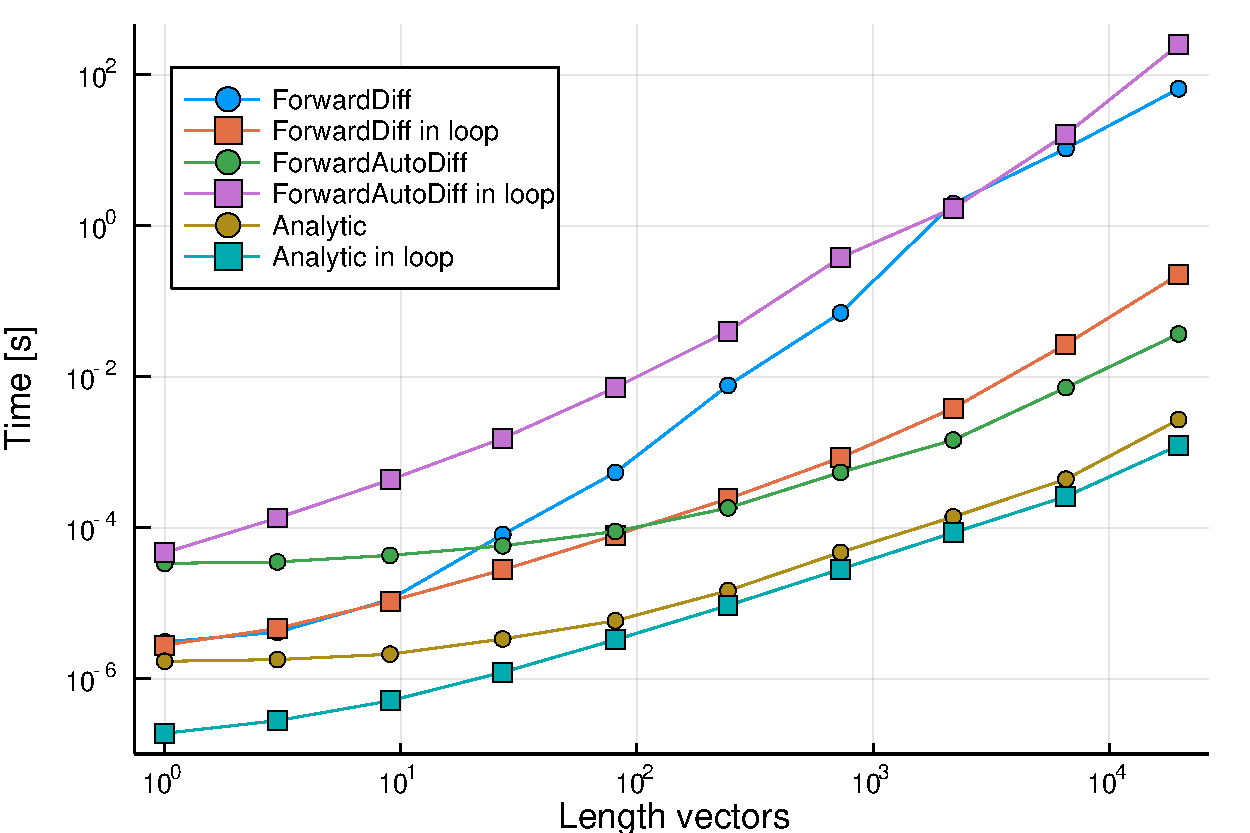
\includegraphics[width = 0.9\textwidth]{figures/benchmark_ad_in_loop.pdf}
    \caption{Time spent calculating the value and gradient of $f$ in \eqref{eq:benchmarkFunction} as                         a function of length of the input vectors. \todo[inline]{få plottene som tilhører samme metode i samme farge}}
    \label{fig:adInLoop}
\end{figure}
We can start by observing that the ForwardAutoDiff implementation is clearly not optimized for evaluating the vector function scalar by scalar as it is the slowest method we have tested so far for all vector lengths. The next interesting observation is that we can make ForwardDiff's evaluation of the vector function much more efficient. When using the method in \texttt{benchmarkADinLoop} we almost achieve the same test results as ForwardAutoDiff. Although, what is important to mention here is that with the approach in \texttt{benchmarkADinLoop} we only obtain the gradient of the function and not the Jacobian. In the particular case of the function $f$ in \eqref{eq:benchmarkFunction}, the Jacobian will only be a diagonal matrix with the gradient of $f$ on the diagonal, but if we would evaluate a function like in \eqref{eq:differenceFunction}, this approach would not work. Hence, although we almost manage to obtain the same performance in ForwardDiff as we have in ForwardAutoDiff, it comes with a cost that some type of functions cannot be evaluated. The implementation necessary to work around this and obtain the Jacobian with ForwardDiff and \texttt{benchmarkADinLoop} will slow the computation down and for a vector function with large input vectors, ForwardAutoDiff is a better approach. 

Other than this, what is interesting to see is that the evaluation of the analytical solution in a loop is faster than its vectorized counterpart. Here, Julia shows a real strength compared to MATLAB, where a function evaluation like for the vector function $f$ will be much slower in a loop than vector multiplication.
\begin{figure}[htb]
    \centering
    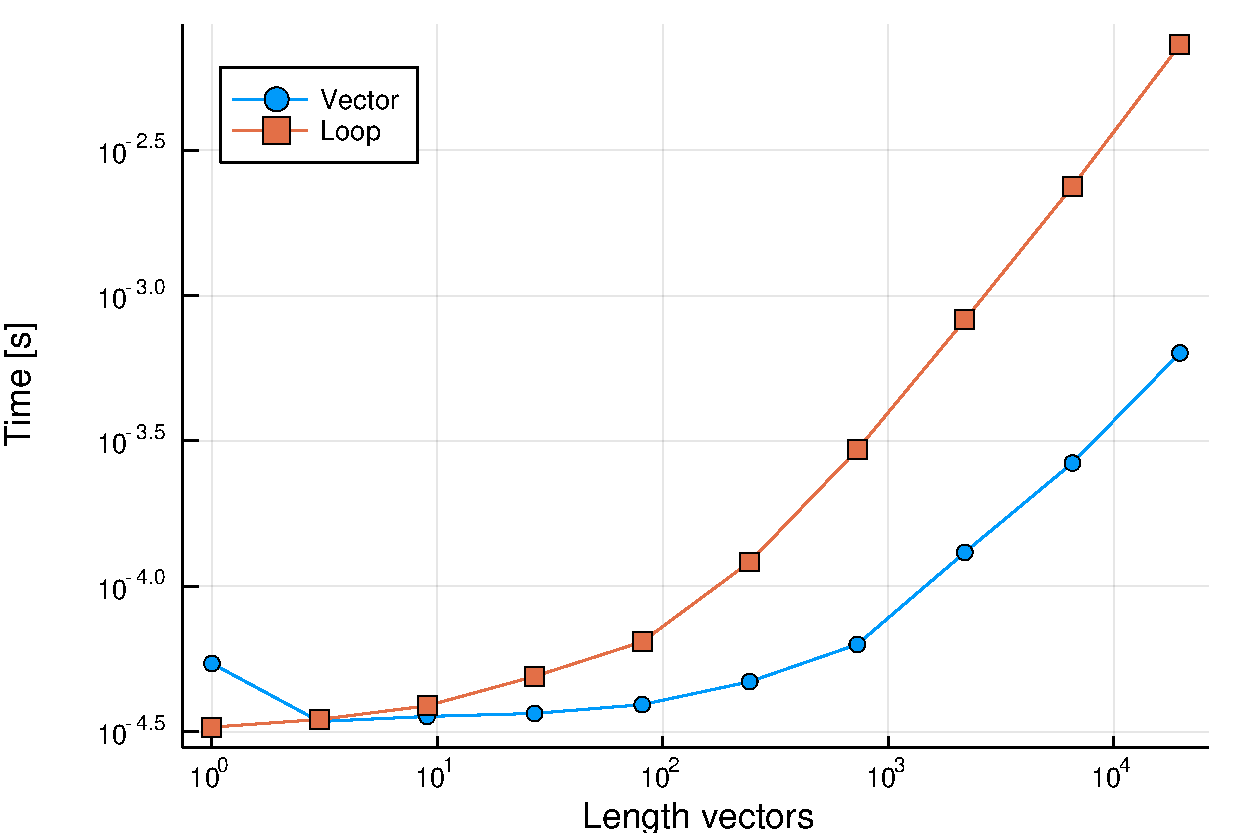
\includegraphics[width = 0.9\textwidth]{figures/benchmark_matlab_multiplication.pdf}
    \caption{Time spent evaluating the analytic functions $f$, $f_x$, $f_y$ and $f_z$ from \eqref{eq:benchmarkFunction} as a function of length of the input vectors in MATLAB.}
    \label{fig:matlabMultiplication}
\end{figure}
\autoref{fig:matlabMultiplication} shows how much time MATLAB uses to evaluate the analytic functions $f$, $f_x$, $f_y$ and $f_z$ from \eqref{eq:benchmarkFunction} as vector multiplication or in a for loop just like the analytic graphs in \autoref{fig:adInLoop} where Julia did the same. And where the vector multiplication and for loop scale equally good in Julia, but the for loop actually perform better, MATLAB's for loops scale much worse than the vector multiplication. Even though this does not confirm that the developers of Julia have managed to create a language with similar mathematical syntax as MATLAB, but where for loops are ok to use, it gives indications that it might be the case.

\section{Flow Solver With Automatic Differentiation}
\label{sec:FlowSolver}
To test Julia's AD tools in a real world application I have implemented an example taken from the MATLAB Reservoir Simulation Toolbox (MRST) and implemented it in Julia. MRST is primary developed by the Computational Geosciences group in the department of Mathematics and Cybernetics at SINTEF Digital \emph{\cite{mrstHomepage}}. According to MRST's homepage, "MRST is not primarily a simulator, but is mainly intended as a toolbox for rapid prototyping and demonstration of new simulation methods and modelling concepts". So although most of the tools and simulators in MRST are very efficient and perform well - if you are to simulate more heavy simulation they recommend to use the Open Porous Media (OPM) Flow simulator \emph{\citep{OPM}}. OPM is a toolbox to build simulations of porous media processes and are mainly written in C++ and C. Here, the differences between the languages become clear. As MATLAB with its easy to use mathematical syntax is a great language to quickly make prototypes and demonstrations of simulations, it is failing somewhat when it comes to computational speed. But where MATLAB fails in computational speed, C++ and C are two very fast languages. The problem with C++ and C is that these languages are not built for numerical analysis, hence it takes longer time to create the simulations. This is where Julia comes in. As the founders of Julia said, Julia is meant to be a language as familiar to mathematical notations as MATLAB, but as fast as C. Hence it is interesting to figure out how Julia can perform compared to MRST.

To compare different AD implementations in Julia and MATLAB I have implemented MRST's tutorial called "Single-phase Compressible AD Solver" from \texttt{flowSolverTutorialAD.m} \emph{\citep{flowSolverADExample}} in Julia. The example is made as an introduction to how AD can be used in MRST, hence it is a good example to use to compare the implementation of AD in MATLAB and Julia. 

The example consist of modelling how the pressure drops within a rectangular reservoir measuring $200\times 200 \times 50 \text{m}^3$ when we have a well that that is producing oil. That it is a single-phase solver only means that we do not have different phases of fluid, like liquid and gas, present during the simulation. As the purpose of this example is to compare the AD tools in MATLAB and Julia and not the process of solving the problem, including setting up the grid and other necessary variables, some of the initialization and plotting have been performed in Julia by calling code from MRST. This has been done by using the package MATLAB.jl \emph{\citep{MATLAB.jl}}. This package allows calling MATLAB functions from Julia and retrieve the output variables. This is done by the function call
\lstinputlisting{code/mxcall.jl}
where we have three input parameter and two output parameters. We have to specify the number of output parameters after the MATLAB function name.  By calling MATLAB from Julia we can use MRST's \texttt{G = computeGeometry(...)} function to set up the grid for the simulation. The grid of the reservoir can be seen in \autoref{fig:flowSolverGrid}. The variable \texttt{G} that contains the grid properties is now a structured array (struct) that has all the information on cells, facets, vertices and nodes that we need to make the discrete divergence and gradient operators as explained in \autoref{sec:ApplicationsAD}. 

Next, we define the properties of the rock. In an oil reservoir, the oil lies inside porous rock and hence the properties of the rock will affect the flow of the oil. The amount of oil we can have inside the rock is measured as pore volume. First, we make a new variable \texttt{rock} that contains parameters that describe the rock's ability to store and trasmit fluids for each cell with the function  \texttt{rock = makeRock(...)}. Then we say that in our model the rock is compressed constantly as a function of pressure and we obtain the analytic solution for the pore-volume as a function of pressure
\begin{equation}
    pv(p) = \text{pv}_r \exp[c_r\cdot(p-p_r)],
    \label{eq:poreVolume}
\end{equation}
where pv$_r$ is the rock pore-volume properties in a cell at a reference pressure $p_r$ and $c_r$ is a constant controlling how the rock is compressed. The pore-volume of the rock as a function of pressure values are visualized in \autoref{fig:flowSolverPoreVolume}. The graph shows that for a cell with volume $1000\text{m}^3$ there is approximately room for $600\text{m}^3$ oil.

Since we assume that the oil have a constant compressibility, the density of the oil is given as an analytic function of pressure 
\begin{equation}
    \rho(p) = \rho_r\exp[c\cdot(p-p_r)],
    \label{eq:pressureSolverDensity}
\end{equation}
where in our case $\rho_r = 850\text{kg}/\text{m}^3$ and $c$ is a constant controlling how fast the oil is compressed. The density of the fluid as a function of pressure is plotted for some pressure values in \autoref{fig:flowSolverDensity}.
\begin{figure}[htb]
    \centering
    \begin{subfigure}[t]{0.48\textwidth}
        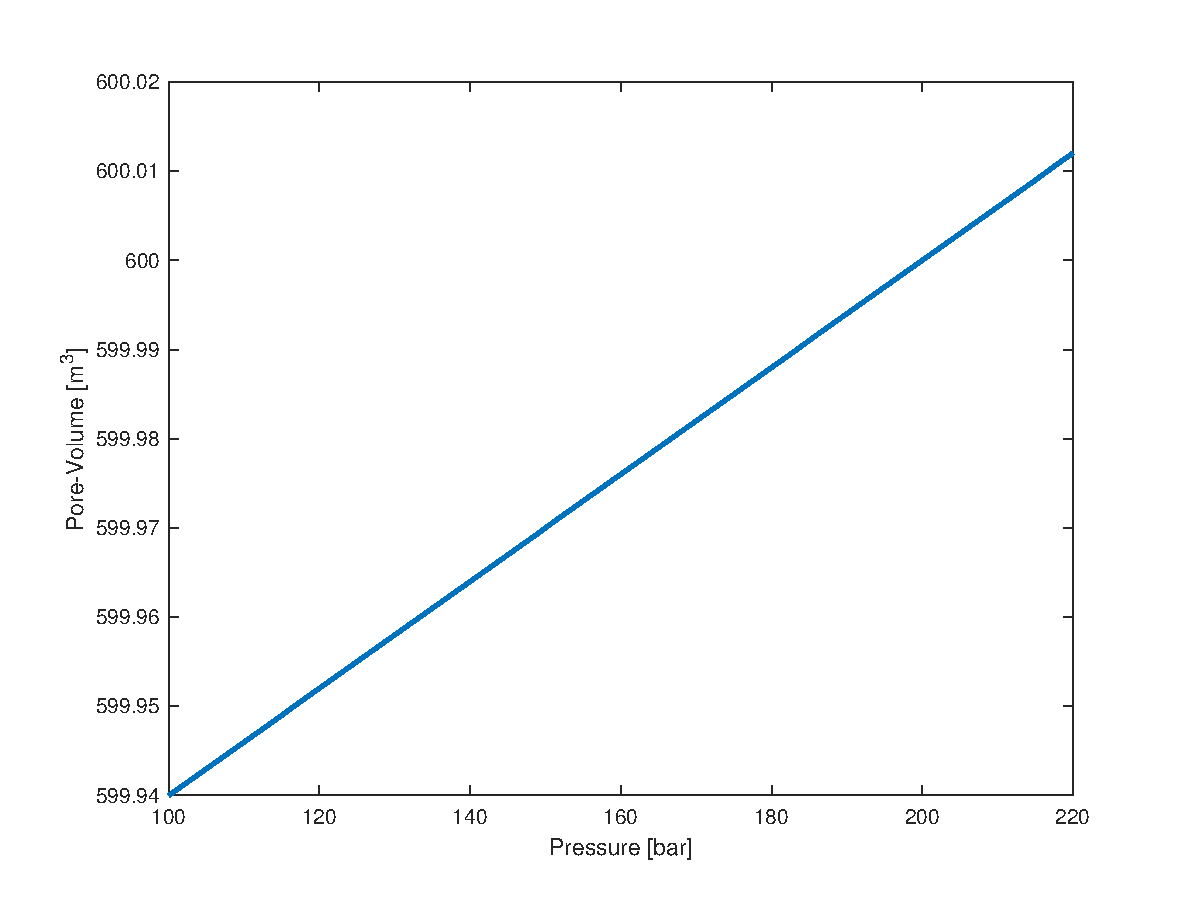
\includegraphics[width=\textwidth]{figures/flow_solver_pore-volume.eps}
        \caption{The pore-volume of the rock in a cell as a function of pressure.}
        \label{fig:flowSolverDensity}
    \end{subfigure}
    \begin{subfigure}[t]{0.48\textwidth}
        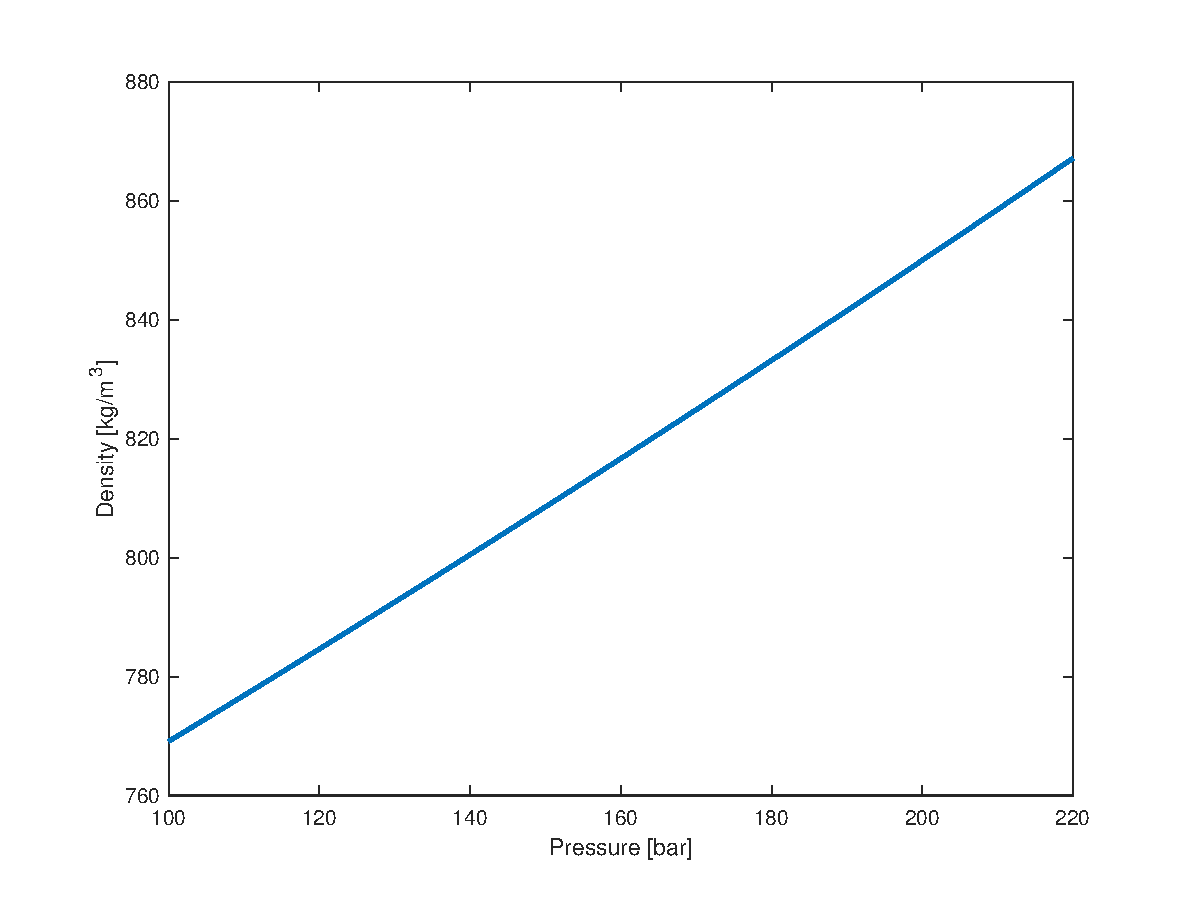
\includegraphics[width=\textwidth]{figures/flow_solver_density.eps}
        \caption{The density of the oil in the reservoir plotted as a function of pressure}
        \label{fig:flowSolverPoreVolume}
    \end{subfigure}
    \caption{\todo[inline]{Burde den ikke være motsatt? Plass til mindre olje jo høyere trykket er?}}
\end{figure}

The initial pressure in the reservoir is calculated by solving the nonlinear ODE
\begin{equation*}
    \frac{dp}{dz} = g\cdot \rho(p), \quad p(z = 0) = p_r = 200\text{bar} 
\end{equation*}  
for the fluid density given by $\rho(p) = \rho_r\cdot\exp\big(c\cdot(p-p_r\big)$ for the same constants $\rho_r$ and $c$ as in \autoref{eq:pressureSolverDensity}. The well is then inserted by removing 8 grid elements using the \texttt{addWell(...)} function. The grid with initial pressure and well can be seen in \autoref{fig:flowSolverGridWithWell}.
\begin{figure}[htbp]
    \centering
    \begin{subfigure}[t]{0.48\textwidth}
        \centering
        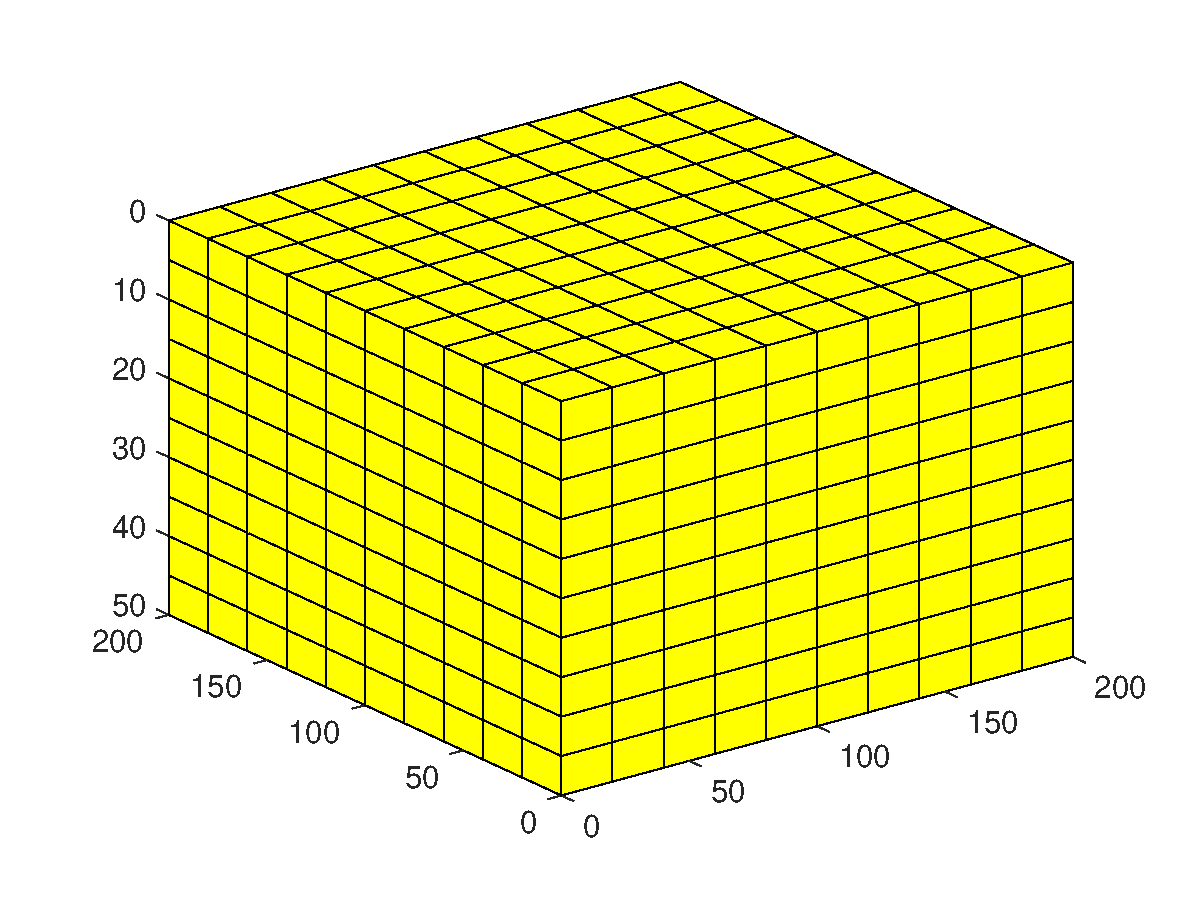
\includegraphics[width = \textwidth]{figures/flowSolver_grid.eps}
        \caption{Uniform $10\times 10 \times 10$ grid of the $200\times 200 \times 50 \text{m}^3$ big reservoir.}
        \label{fig:flowSolverGrid}
    \end{subfigure}
    \hfill
    \begin{subfigure}[t]{0.48\textwidth}
        \centering
        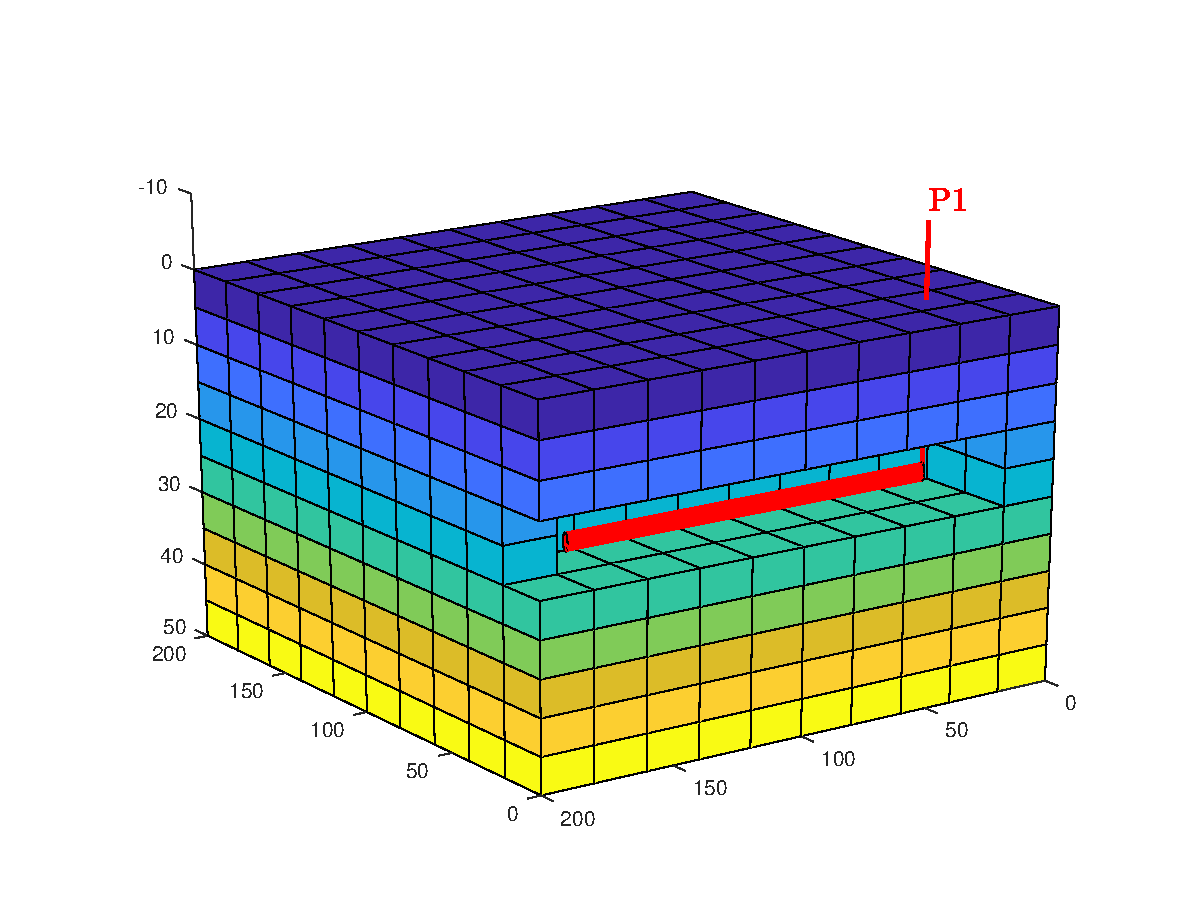
\includegraphics[width = \textwidth]{figures/flowSolver_gridWithWell.eps}
        \caption{Reservoir grid plotted with initial pressure and well P1. Pressure is given in bar. The well has replaced 8 grid elements. Some grid elements are removed to give a better visualization of the well.}
        \label{fig:flowSolverGridWithWell}
    \end{subfigure}
    \caption{}
\end{figure}

After initializing the grid we want to define the discrete gradient and divergence operators as well as the transmissibilities as explained in equation \eqref{eq:transmissibility}. This is done by exploiting that we have all the necessary information about the grid properties, such as the cells centroid coordinates, facets areas and so on, stored in the struct \texttt{G}. In \texttt{rock} we have stored the permeability inside each cell that will affect the flux through each facet. With all this information we can now obtain the transmissibilities \texttt{T} and the discrete operators
\lstinputlisting{code/grad_and_div.jl}

\begin{wrapfigure}{r}{5.5cm}
    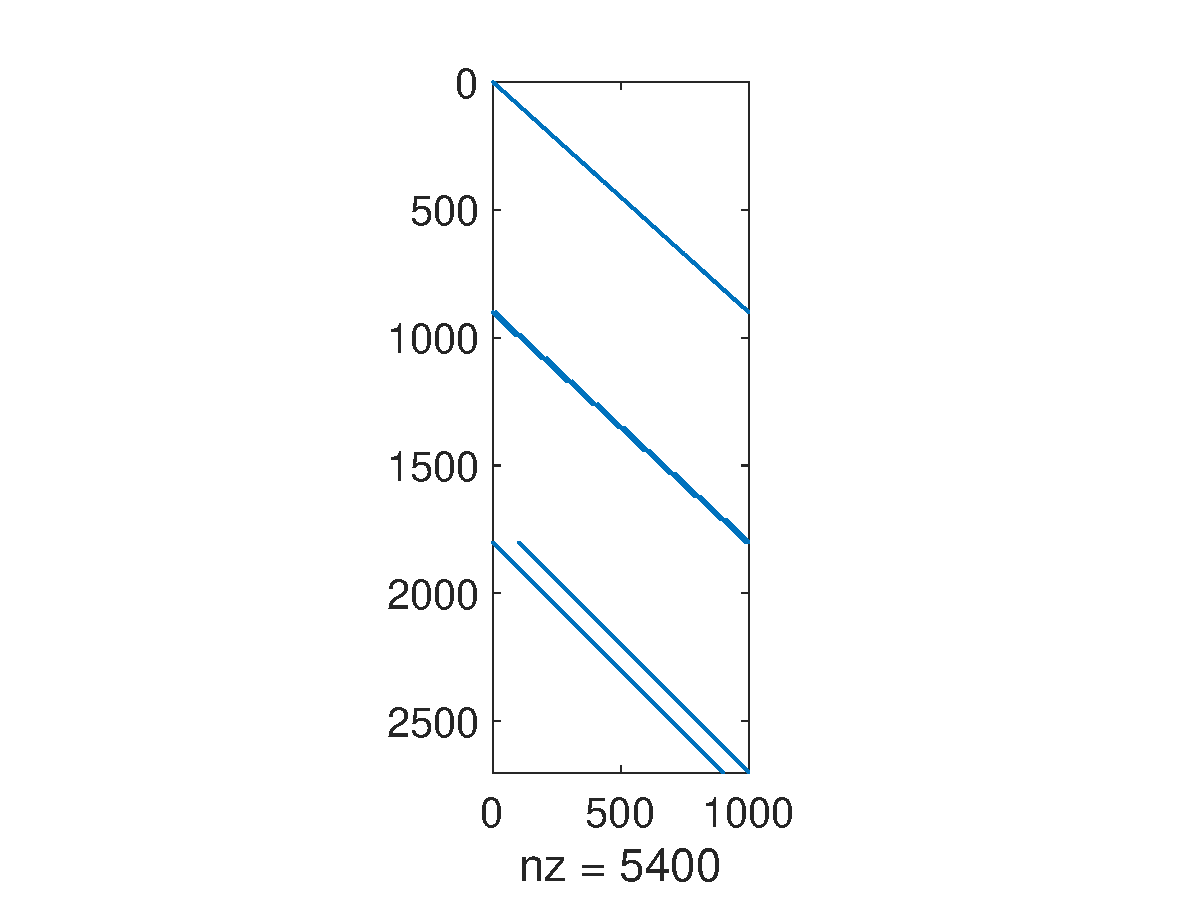
\includegraphics[width=\linewidth]{figures/flowSolver_discrete_operators_C.eps}
    \caption{Structure of discrete operator \texttt{C}.}
    \label{fig:discreteOperatorsC}
\end{wrapfigure}
The matrix C in the discrete operators are created such that when it is multiplied by the pressure $p$, the result becomes the pressure difference between two adjacent cells like defined in \eqref{eq:discreteGradient}. The matrix C is stored as a sparse matrix, and the reason why is clear from \autoref{fig:discreteOperatorsC}, which shows the sparse  structure of C. The divergence operator is made using the fact that in the continuous case, the gradient operator is the adjoint of the divergence operator
\begin{equation*}
    \int_\Omega p\nabla \cdot \vec{v} d\Omega + \int_\Omega \vec{v}\nabla p d\Omega = 0.
\end{equation*}
This holds for the discrete case as well \emph{\citep{lieMrstUrl}}, and hence the adjoint of \texttt{C} is the negative transpose of \texttt{C}.

Now, we have all the ingredients to set up the governing equations for the flow in the reservoir. We use a finite volume method to discretize in space, like explained in \autoref{sec:ApplicationsAD}, and a backward Euler method to discretize in time. In the end we want all the equations we want to solve on residual form, $\boldsymbol{F}(\boldsymbol{x}) = 0$ such that we can use the Newton-Raphson method described in equation \eqref{eq:newtonRaphsonVector} to solve the system. As there are multiple equations that will be a part of the residual function $\boldsymbol{F}(\boldsymbol{x})$, we define them separately first. One of the advantages of defining the discrete gradient and divergence operators are that the continuous and discrete forms of the equations look very similar. Hence I will first state the continuous version of the equation and then the discrete, such that it is easy to see how similar they look. We start by defining Darcy's law which explains how the the oil will flow through the pourous rock

\todo[inline]{Herfra og nedover har jeg ikke 100\% kontroll på om det jeg har skrevet er korrekt. Kan hende det er lettest å få bekreftelse eventuelt rette opp på sintef.}
\begin{equation*}
    \vec{v} = - \frac{k}{\mu}(\nabla p - \vec{g}\rho).
    \label{eq:pressSolverDarcy}
\end{equation*}
Here, $k$ is the permeability that we have saved in the \texttt{rock} variable and $\mu$ is the viscosity of the oil.
The corresponding discrete equation that we call \text{flux} is given by 
\lstinputlisting{code/flux.jl}
Here, T is the transmissibilities that contain $k$ and the properties of the grid. Since two adjacent cells can have different values of $\rho$, we use the  average for the two cells. \texttt{gradz} is the gradient of the cell centroid's $z$-value. This makes sure that if the cells lie next to each other in the horizontal plane, the flux will not depend on $g$. When \texttt{flux} is defined, we define the continuity equation in the continuous case
\begin{equation*}
    \frac{\partial}{\partial t}(\phi\rho)(p) + \nabla\cdot(\rho\vec{v}) = q,
\end{equation*}
where $\phi$ is the porosity of the rock. Since we will handle the well later, the source term $q$ representing injection or production fluids is set to zero. In the corresponding discrete case we get the function
\lstinputlisting{code/presEq.jl}
where \texttt{pv} is the pore-volume of the rock given in Equation \eqref{eq:poreVolume} and $p0$ is the pressure at the previous time step. 

In addition, we need a few equations to represent the flow inside the wellbore. This flow will be the production term $q$ we ignored in the derivation of the \texttt{presEq} function. The standard model is to assume that the pressure is in hydrostatic equilibrium inside the wellbore, so that the pressure in a perforated cell (i.e., a cell in which the wellbore is open to the reservoir rock) is given as a hydrostatic difference from the pressure at a datum point (the bottom-hole pressure), typically given at the top of the reservoir. That is, the pressure in a perforated cell $c$ is given by
\begin{equation*}
p_c = p_{bh} + g (z_c - z_{bhp})\rho.    
\end{equation*}
In the discrete case this is given by the function \texttt{p_conn}
\lstinputlisting{code/p_conn.jl}
The pressure drop near the well usually takes place on a much shorter length scale than the size of a grid cell, and is usually modelled through a semi-analytical expression that relates flow rate to the difference between the reservoir and wellbore pressures. Hence the analytic expression for the production in a perforated cell is given by
\begin{equation*}
    q = (\rho\mbox{WI}/\mu)(p_c - p_r)
\end{equation*}

\lstinputlisting{code/q_conn.jl}

\lstinputlisting{code/rateEq.jl}
To control the well, we can either set total inflow or outflow of the well (evaluated at surface pressure) to be constant, or set the datum (bottom-hole) pressure as constant. In either case, we will wish to compute the other (i.e., if pressure is given, we determine the surface rate, and vice versa). Herein, we assume pressure to be given
\lstinputlisting{code/ctrlEq.jl}

When all the governing equations are defined, we merge them into one large residual vector function $\boldsymbol{F}(\boldsymbol{x})$. Here, $\boldsymbol{x}\in\Re^{1002}$, where the first 1000 elements are the pressure at the different nodes, element 1001 will be the pressure at the datum point inside the well (\texttt{bhp}), and element 1002 is the surface fluid rate\texttt{qS}. Now, if we start by defining \texttt{p}, \texttt{bhp} and \texttt{qS} as AD-variables, $\boldsymbol{F}$ will also be an AD-variable and we will have the Jacobian of the residual vector function $\boldsymbol{F}$. This means we can solve the equations using the Newton-Raphson method \eqref{eq:newtonRaphsonVector}. A pseudo code of how we solve the system can be seen below.
\lstinputlisting{code/press_solver_main_loop.jl}
If we simulate how the pressure in the reservoir will decay during one year, we will get the result displayed in \autoref{fig:flowSolverResult}.
\begin{figure}[htbp]
    \centering
    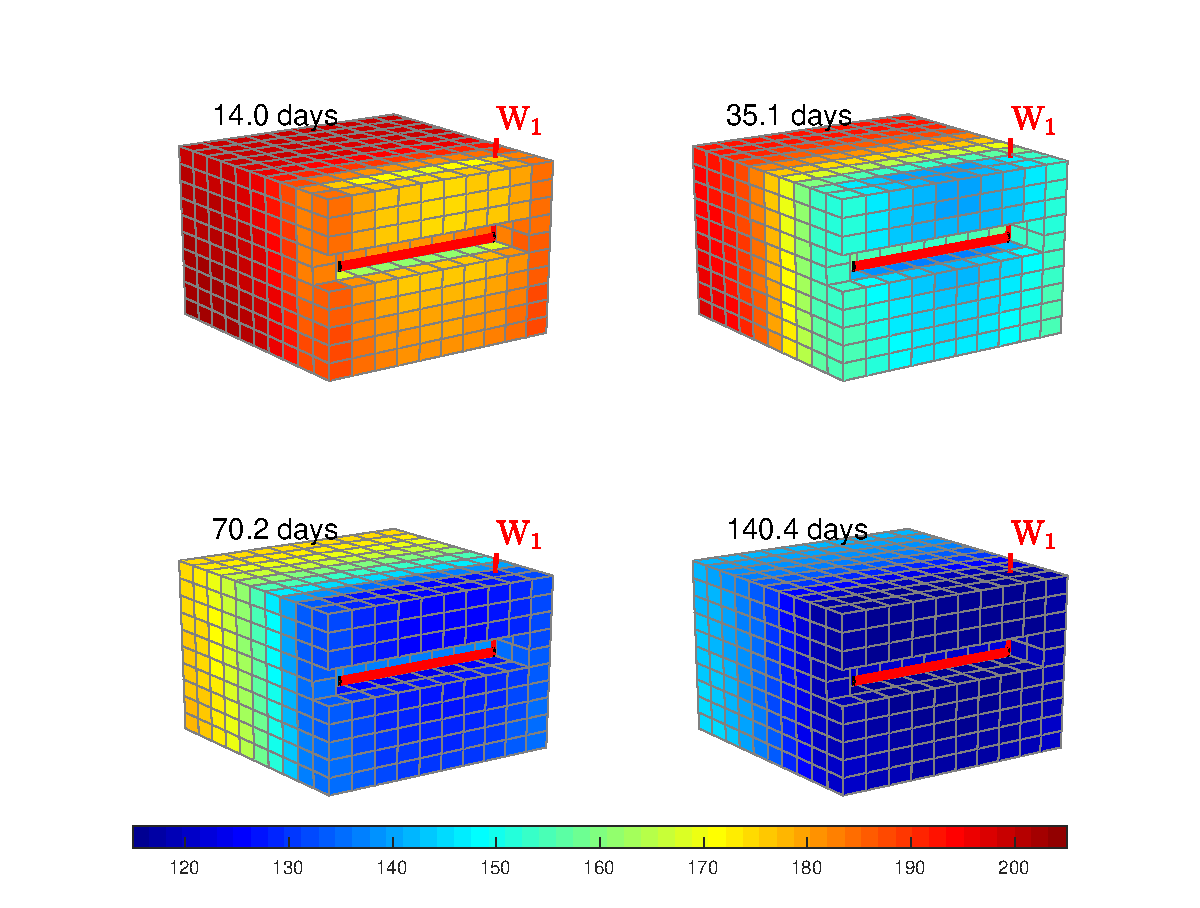
\includegraphics[width = 0.9\textwidth]{figures/flowSolver_result.eps}
    \caption{The pressure in the reservoir displayed at four different times. Pressure is given in bar.}
    \label{fig:flowSolverResult}
\end{figure}
Note the different intervals for the color bar in \autoref{fig:flowSolverResult} compared to \autoref{fig:flowSolverGridWithWell}. With the current color bar interval, at initial state, the whole reservoir will be displayed red. Hence, we can see how the reservoir from the beginning being approximately 200 bar everywhere, begins with the largest pressure decay close to the well, but after some time, the oil is pushed towards the well by the pressure differences and the pressure begins to decay also furthest away from the well. 

\autoref{fig:flowSolverProduction} shows the development of the production rate and the average pressure inside the reservoir. We can see how the production rate follows the average pressure inside the reservoir and that after some time it approaches zero. This phase is what is called primary production. In primary production, the pressure in the reservoir is so high that there is no need to pump the oil out, the pressure difference does all the work. After some time, we can see that the pressure becomes too low and the production decreases. When this happens, we transit to what is called secondary production. To retrieve more oil from the reservoir we need to apply extra pressure inside the reservoir. This can for example consist of injecting water or gas into the reservoir. This is called the secondary production. More details about how this work can be found in \emph{\citep{lieMrstUrl}}, but the main idea here is that to keep up the production and fully exploit the resources in the reservoir, we need to apply external pressure. And to do this in the best possible way, it is important to be able to simulate how the pressure evolves inside the reservoir. This is a simple example of how that can be done elegantly with governing equations on residual form and AD.
\begin{figure}[htbp]
    \centering
    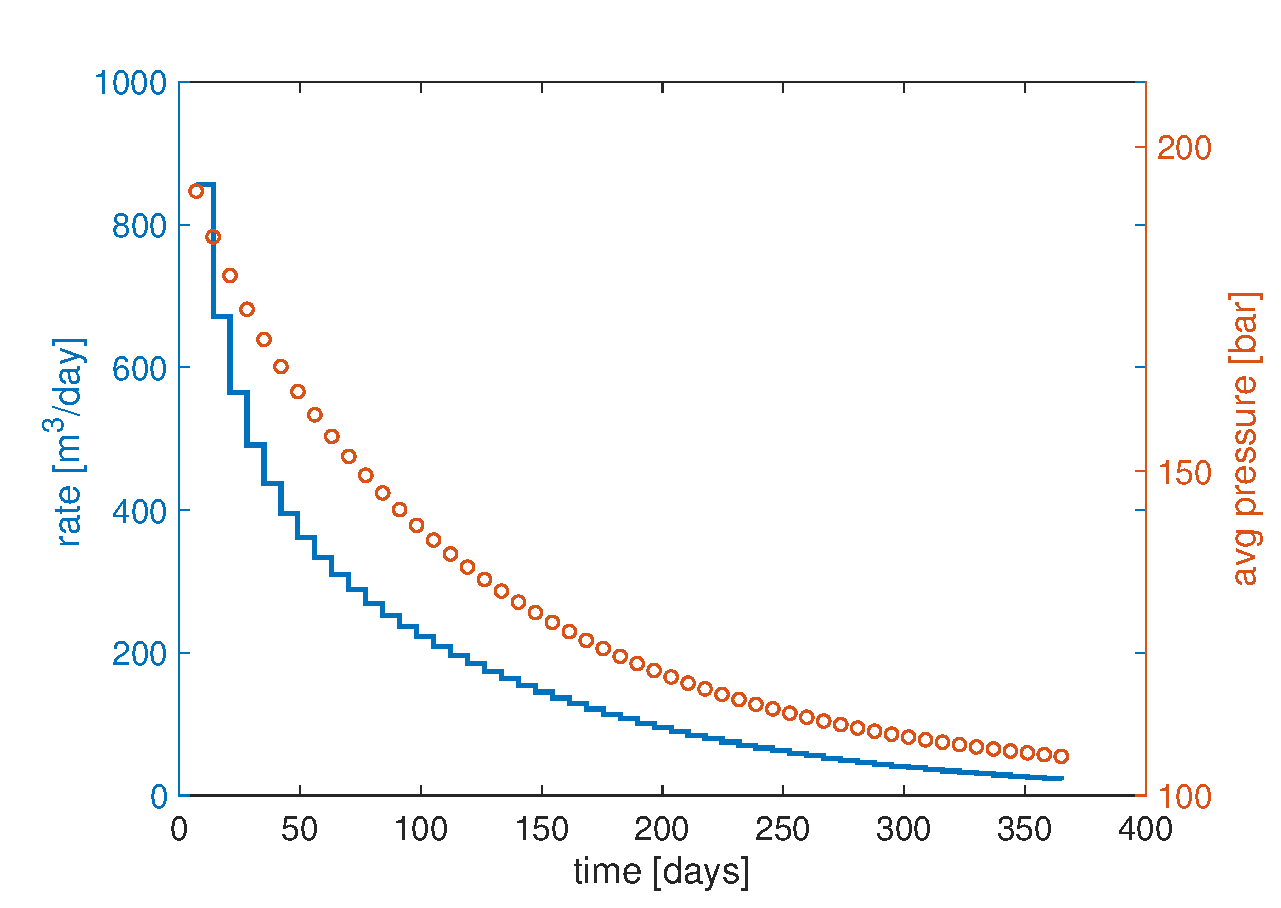
\includegraphics[width = 0.9\textwidth]{figures/flow_solver_production.eps}
    \caption{The production rate and the average pressure in the reservoir as a function of time.}
    \label{fig:flowSolverProduction}
\end{figure}

When it comes to solving the residual equations with the Newton-Raphson method, it is interesting to have a look at how the Jacobian of $\boldsymbol{F}$ looks like. \autoref{fig:flowSolverJacobian} shows the structure of the Jacobian. The first impression is that the matrix is very sparse. Except from a few nonzero points in row 1001 and column 1001 because of the well, the Jacobian consist of 7 diagonals (can look like 5 from perspective) with nonzero elements and the rest of the elements are 0. As we also can see from the figure, there are only 6419 non-zero out of more than 1 million matrix elements. It is clear that storing the full $1002\times 1002$ matrix will be very inefficient.

As explained in \autoref{sec:ApplicationsAD}, the different types of AD mentioned store the Jacobians differently. In ForwardAutoDiff and MRST's implementations of AD, the Jacobians are stored as a list of sparse matrices where each Jacobian element in the list is the Jacobian with respect to one primary variable. In this example this is much more efficient than storing the full $1002\times 1002$ Jacobian as ForwardDiff does.
\begin{figure}[htbp]
    \centering
    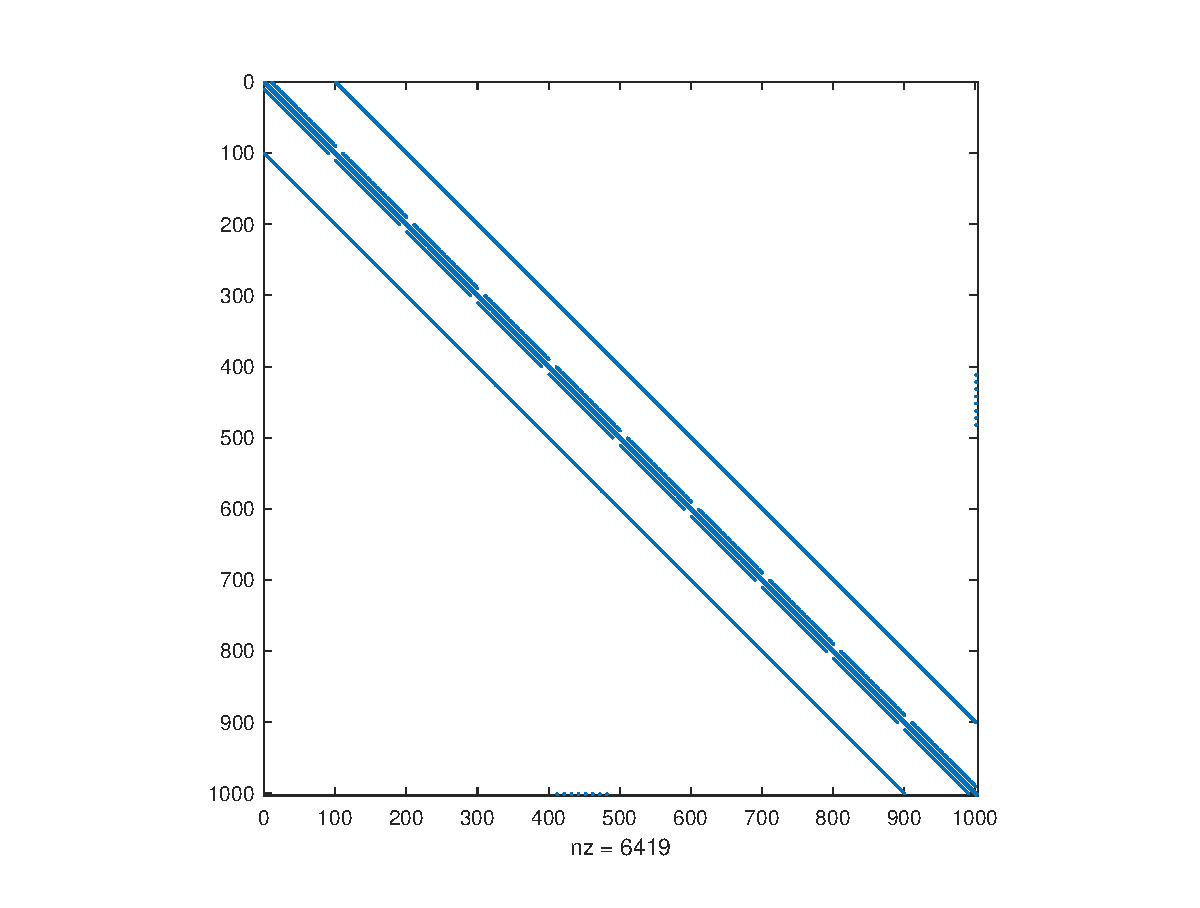
\includegraphics[width = 0.9\textwidth]{figures/flowSolver_Jacobian.eps}
    \caption{Structure of the $1002\times 1002$ Jacobian of the governing equations. There are 6419 non-zero elements.}
    \label{fig:flowSolverJacobian}
\end{figure}
The difference in implementation of the Jacobian should make a big impact on the computation time for this problem. To benchmark the different methods we need to do some extra work to make sure that it is actually the AD we benchmark and not other parts of the code. This is especially important for the code running in Julia, since when we call MATLAB from Julia it will be a lot of overhead. This means that the setup of the discrete gradient and divergence operators will take longer when done in MATLAB called from Julia, than when we do it directly in MATLAB. If we want to run the full simulation it is not possible to separate the AD part fully, but if we only benchmark the main-loop containing the Newton-Raphson method, AD will be a dominating part of the computations together with the linear solver \texttt{f.jac\textbackslash f.val}. This means we at least will get an indication of how well the AD tools perform compared to each other. To see how the different methods scale as the discretization becomes finer and the system we solve grow, I have benchmarked three different discretizations. The first is the original setup with 10 cells in spatial direction $x$, $y$, and $z$. This gives a total number of 1000 cells in the reservoir. Then, I have also tested the implementations for 20 and 30 cells. The time spent solving the system for the different methods can be seen in \autoref{tab:FlowSolverSpeedTest}.
\begin{table}[htb]
    \centering
    \caption{Table with speed benchmarks of different AD methods solving the "Single-Phase Compressible AD Solver" for different discretizations.}
    \label{tab:FlowSolverSpeedTest}
    \begin{tabular}{cccc}
    \textbf{Number of cells} & \textbf{ForwardDiff} & \textbf{ForwardAutoDiff} & \textbf{MRST}\\ \hline
         $10\times10\times10$ & 71.5s & 2.3s & 1.9s \\  
         $20\times20\times20$ & ~ & 31.9s & 23.4s \\ 
         $30\times30\times30$ & ~ & 188.8s & 147.8s\\ \hline
    \end{tabular}
\end{table}
For 10 cells in each spatial direction it is clear that what we assumed based on the structure of the Jacobian in \autoref{fig:flowSolverJacobian} is true. The ForwardDiff method takes much longer time than ForwardAutoDiff and MRST. Since ForwardDiff already spends over a minute for $10\times 10\times 10$ cells, it is omitted for finer discretizations. \autoref{tab:FlowSolverSpeedTest} shows that the trend with MRST being a bit faster than ForwardAutoDiff continues for finer discretizations. 
\todo[inline]{Er det relevant å ha med kode i Appendix? Eventuelt levere kode ved siden av?}